% ============================================================
% CHAPITRE 9 : OPTIMISATIONS ET PERSPECTIVES
% ============================================================

\chapter{Optimisations et Perspectives Avancées}

\section{Introduction}

Ce chapitre explore les optimisations avancées permettant de réduire le coût, la consommation énergétique et le temps de réponse du système DMS, ainsi que les approches innovantes pour améliorer ses performances. Ces optimisations sont essentielles pour le déploiement en production sur des ECU automobiles réels.

\section{Optimisation de l'Architecture CNN}

\subsection{Quantification des Modèles}

La \keyword{quantification} consiste à réduire la précision des poids et des activations du CNN de 32 bits (FP32) à 8 bits (INT8), permettant une réduction significative de la taille du modèle et une accélération de l'inférence.

\subsubsection{Quantification Post-Entraînement (PTQ)}

La quantification post-entraînement convertit les poids après l'entraînement :

\begin{equation}
q = \text{round}\left(\frac{r - r_{\min}}{r_{\max} - r_{\min}} \times (2^b - 1)\right)
\label{eq:quantization}
\end{equation}

où $r$ est la valeur en virgule flottante, $q$ la valeur quantifiée, et $b = 8$ le nombre de bits.

\begin{lstlisting}[style=pythonstyle, caption={Quantification du modèle avec PyTorch.}, label={lst:quantization}]
import torch.quantization as quant

def quantize_model(model, calibration_data):
    """
    Quantifie le modele CNN en INT8.
    
    Reduction attendue:
    - Taille: ~4x (FP32 -> INT8)
    - Vitesse: ~2-3x sur CPU ARM
    - Precision: <1% de perte
    """
    # Configuration de la quantification
    model.eval()
    model.qconfig = quant.get_default_qconfig('fbgemm')
    
    # Preparation du modele
    model_prepared = quant.prepare(model)
    
    # Calibration avec des donnees representatives
    with torch.no_grad():
        for data in calibration_data:
            model_prepared(data)
    
    # Conversion en modele quantifie
    model_quantized = quant.convert(model_prepared)
    
    return model_quantized
\end{lstlisting}

\subsubsection{Impact de la Quantification}

\begin{table}[H]
\centering
\caption{Impact de la quantification sur le EyeStateCNN.}
\label{tab:quantization_impact}
\renewcommand{\arraystretch}{1.3}
\begin{tabular}{|l|c|c|c|}
\hline
\rowcolor{stellantisblue!15}
\textbf{Métrique} & \textbf{FP32} & \textbf{INT8} & \textbf{Gain} \\
\hline
Taille du modèle & 1.55 Mo & 0.39 Mo & $\times 4.0$ \\
\hline
Temps d'inférence (CPU) & 8.7 ms & 3.2 ms & $\times 2.7$ \\
\hline
Consommation mémoire & 12 Mo & 3.5 Mo & $\times 3.4$ \\
\hline
Précision & 95.2\% & 94.8\% & $-0.4\%$ \\
\hline
\end{tabular}
\end{table}

\subsection{Pruning (Élagage)}

Le \keyword{pruning} supprime les connexions (poids) les moins significatives du réseau :

\begin{equation}
\mathbf{W}_{\text{pruned}}[i, j] = \begin{cases}
    \mathbf{W}[i, j] & \text{si } |\mathbf{W}[i, j]| > \tau \\
    0 & \text{sinon}
\end{cases}
\label{eq:pruning}
\end{equation}

où $\tau$ est le seuil de pruning. Un taux de pruning de 50\% permet de réduire les opérations de moitié avec une perte de précision minimale.

\begin{lstlisting}[style=pythonstyle, caption={Pruning structuré du CNN.}, label={lst:pruning}]
import torch.nn.utils.prune as prune

def prune_model(model, amount=0.5):
    """
    Applique le pruning non-structure au modele.
    
    Args:
        model: Modele PyTorch
        amount: Fraction des poids a supprimer (0.5=50%)
    """
    for name, module in model.named_modules():
        if isinstance(module, torch.nn.Conv2d):
            prune.l1_unstructured(module, 
                name='weight', amount=amount)
        elif isinstance(module, torch.nn.Linear):
            prune.l1_unstructured(module, 
                name='weight', amount=amount)
    
    return model
\end{lstlisting}

\subsection{Conversion ONNX pour le Déploiement}

Le format \keyword{ONNX} (\textit{Open Neural Network Exchange}) permet de déployer le modèle sur différentes plateformes embarquées :

\begin{lstlisting}[style=pythonstyle, caption={Export du modèle au format ONNX.}, label={lst:onnx_export}]
def export_to_onnx(model, output_path='model.onnx'):
    """
    Exporte le modele PyTorch au format ONNX.
    
    Compatibilite:
    - TensorRT (NVIDIA)
    - OpenVINO (Intel)
    - ONNX Runtime (universel)
    - Edge TPU (Google Coral)
    """
    dummy_input = torch.randn(1, 1, 24, 24)
    
    torch.onnx.export(
        model,
        dummy_input,
        output_path,
        export_params=True,
        opset_version=11,
        do_constant_folding=True,
        input_names=['input'],
        output_names=['output'],
        dynamic_axes={
            'input': {0: 'batch_size'},
            'output': {0: 'batch_size'}
        }
    )
\end{lstlisting}

\subsection{Architecture MobileNet pour l'Embarqué}

Le remplacement de l'architecture CNN actuelle par une architecture \keyword{MobileNetV2} \cite{sandler2018} offre des gains significatifs :

\begin{table}[H]
\centering
\caption{Comparaison EyeStateCNN vs MobileNetV2-Tiny.}
\label{tab:mobilenet_comparison}
\renewcommand{\arraystretch}{1.3}
\begin{tabular}{|l|c|c|c|}
\hline
\rowcolor{stellantisblue!15}
\textbf{Métrique} & \textbf{EyeStateCNN} & \textbf{MobileNetV2-Tiny} & \textbf{Gain} \\
\hline
Paramètres & 388\,578 & 42\,150 & $\times 9.2$ \\
\hline
FLOPS & 15.8M & 2.1M & $\times 7.5$ \\
\hline
Taille (FP32) & 1.55 Mo & 0.17 Mo & $\times 9.1$ \\
\hline
Inférence (RPi4) & 8.7 ms & 1.8 ms & $\times 4.8$ \\
\hline
Précision estimée & 95.2\% & 93.5\% & $-1.7\%$ \\
\hline
\end{tabular}
\end{table}

\section{Optimisation de la Consommation Énergétique}

\subsection{Stratégies de Réduction}

\begin{enumerate}[leftmargin=2cm]
    \item \textbf{Traitement adaptatif} : Réduire le FPS lorsque le conducteur est attentif (15 FPS) et augmenter en cas de risque (30 FPS) :
    \begin{equation}
    f_{\text{processing}} = \begin{cases}
        15 \text{ FPS} & \text{si } S_{\max} < 0.2 \\
        30 \text{ FPS} & \text{si } S_{\max} \geq 0.2
    \end{cases}
    \label{eq:adaptive_fps}
    \end{equation}
    
    \item \textbf{Détection paresseuse} : N'exécuter le CNN que si la cascade de Haar détecte un changement significatif par rapport à la dernière image traitée :
    \begin{equation}
    \text{CNN\_required} = \|\mathbf{I}_t - \mathbf{I}_{t-1}\|_F > \delta_{\text{change}}
    \label{eq:lazy_detection}
    \end{equation}
    
    \item \textbf{Mise en veille des capteurs} : Désactiver les LED IR lorsque l'éclairage ambiant est suffisant.
\end{enumerate}

\subsection{Bilan Énergétique}

\begin{table}[H]
\centering
\caption{Bilan énergétique du prototype avec et sans optimisation.}
\label{tab:energy_budget}
\renewcommand{\arraystretch}{1.3}
\begin{tabular}{|l|c|c|c|}
\hline
\rowcolor{stellantisblue!15}
\textbf{Composant} & \textbf{Sans optim. (W)} & \textbf{Avec optim. (W)} & \textbf{Réduction} \\
\hline
Raspberry Pi 4 (CPU) & 6.0 & 4.2 & 30\% \\
\hline
Caméra USB & 0.5 & 0.5 & 0\% \\
\hline
LED IR & 0.4 & 0.2 & 50\% \\
\hline
Module CAN & 0.1 & 0.1 & 0\% \\
\hline
Actionneurs & 0.8 & 0.3 & 62\% \\
\hline
\textbf{Total} & \textbf{7.8 W} & \textbf{5.3 W} & \textbf{32\%} \\
\hline
\end{tabular}
\end{table}

\section{Optimisation du Temps de Réponse}

\subsection{Pipeline Parallèle}

L'utilisation d'un pipeline parallèle avec des threads dédiés permet de réduire la latence :

\begin{figure}[H]
\centering
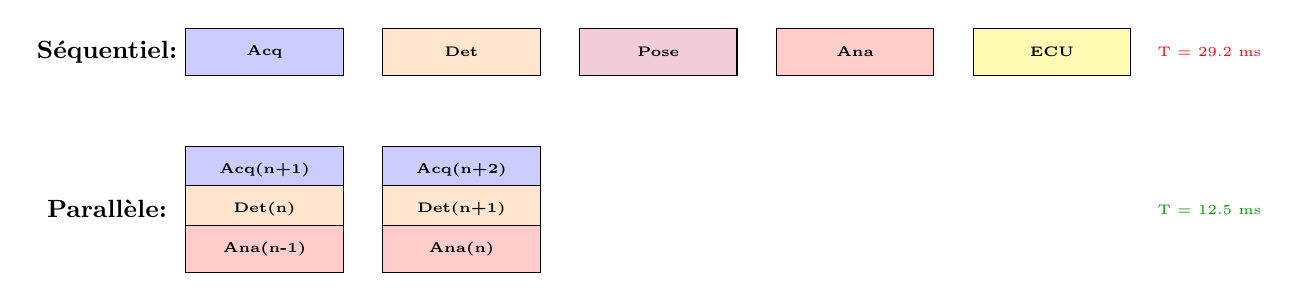
\begin{tikzpicture}[
    stage/.style={rectangle, draw, fill=#1, minimum width=2cm, minimum height=0.6cm, text centered, font=\tiny\bfseries},
    arrow/.style={->, >=stealth}
]
    % Pipeline séquentiel
    \node[font=\small\bfseries] at (-2, 2) {Séquentiel:};
    \foreach \i/\color/\label in {0/blue!20/Acq, 1/orange!20/Det, 2/purple!20/Pose, 3/red!20/Ana, 4/yellow!30/ECU} {
        \node[stage=\color] at (\i*2.5, 2) {\label};
    }
    \node[font=\tiny, color=red] at (12, 2) {T = 29.2 ms};
    
    % Pipeline parallèle
    \node[font=\small\bfseries] at (-2, 0) {Parallèle:};
    
    % Image n
    \node[stage=blue!20] at (0, 0.5) {Acq(n+1)};
    \node[stage=orange!20] at (0, 0) {Det(n)};
    \node[stage=red!20] at (0, -0.5) {Ana(n-1)};
    
    % Image n+1
    \node[stage=blue!20] at (2.5, 0.5) {Acq(n+2)};
    \node[stage=orange!20] at (2.5, 0) {Det(n+1)};
    \node[stage=red!20] at (2.5, -0.5) {Ana(n)};
    
    \node[font=\tiny, color=green!60!black] at (12, 0) {T = 12.5 ms};
    
\end{tikzpicture}
\caption{Pipeline séquentiel vs parallèle.}
\label{fig:pipeline_parallel}
\end{figure}

Le pipeline parallèle réduit la latence effective à celle de l'étape la plus longue (détection Haar : 12.5 ms), permettant un traitement à \textbf{80 FPS} théoriques.

\subsection{Accélération Matérielle}

\begin{table}[H]
\centering
\caption{Options d'accélération matérielle pour le CNN.}
\label{tab:hw_acceleration}
\renewcommand{\arraystretch}{1.3}
\begin{tabularx}{\textwidth}{|l|c|c|X|}
\hline
\rowcolor{stellantisblue!15}
\textbf{Accélérateur} & \textbf{Prix} & \textbf{Gain} & \textbf{Compatibilité} \\
\hline
Google Coral USB & 60 € & $\times 10$ & TensorFlow Lite, Edge TPU \\
\hline
Intel Neural Compute Stick 2 & 80 € & $\times 8$ & OpenVINO, ONNX \\
\hline
NVIDIA Jetson Nano & 130 € & $\times 15$ & CUDA, TensorRT, PyTorch \\
\hline
Hailo-8 & 90 € & $\times 20$ & ONNX, TensorFlow \\
\hline
\end{tabularx}
\end{table}

\section{Approches Avancées pour le DMS}

\subsection{Fusion Multi-Modale}

L'intégration de capteurs supplémentaires améliore la robustesse :

\begin{equation}
S_{\text{fusion}} = \alpha \cdot S_{\text{vision}} + \beta \cdot S_{\text{physio}} + \gamma \cdot S_{\text{véhicule}}
\label{eq:multimodal_fusion}
\end{equation}

avec $\alpha + \beta + \gamma = 1$ et :
\begin{itemize}
    \item $S_{\text{vision}}$ : Score basé sur la caméra (notre système)
    \item $S_{\text{physio}}$ : Score basé sur les capteurs physiologiques (EEG, ECG, GSR)
    \item $S_{\text{véhicule}}$ : Score basé sur le comportement du véhicule (trajectoire, volant)
\end{itemize}

\subsection{Réseaux Temporels (LSTM/Transformer)}

L'ajout d'une couche temporelle capture les dynamiques de la fatigue :

\begin{equation}
\mathbf{h}_t = \text{LSTM}(\mathbf{x}_t, \mathbf{h}_{t-1}, \mathbf{c}_{t-1})
\label{eq:lstm}
\end{equation}

Les avantages des modèles temporels :
\begin{itemize}
    \item Capture des patterns de clignement sur longue durée
    \item Détection des micro-sommeils (fermetures $< 1$s)
    \item Prédiction anticipée de la somnolence
    \item Réduction des faux positifs par lissage temporel
\end{itemize}

\subsection{Détection de Bâillements}

L'analyse de l'ouverture de la bouche via le ratio MAR (\textit{Mouth Aspect Ratio}) :

\begin{equation}
\text{MAR} = \frac{\|p_{51} - p_{59}\| + \|p_{53} - p_{57}\|}{2 \cdot \|p_{49} - p_{55}\|}
\label{eq:mar}
\end{equation}

Un MAR $> 0.6$ maintenu pendant $> 2$ secondes indique un bâillement.

\subsection{Communication V2X}

L'intégration \keyword{V2X} (\textit{Vehicle-to-Everything}) permet :
\begin{itemize}
    \item \textbf{V2I} (\textit{Vehicle-to-Infrastructure}) : Communication avec les panneaux intelligents pour signaler les zones de repos
    \item \textbf{V2V} (\textit{Vehicle-to-Vehicle}) : Avertir les véhicules proches d'un conducteur fatigué
    \item \textbf{V2N} (\textit{Vehicle-to-Network}) : Envoi des données au cloud pour analyse et alerte des services d'urgence
\end{itemize}

\section{Réduction des Coûts de Production}

\begin{table}[H]
\centering
\caption{Stratégies de réduction des coûts pour la production en série.}
\label{tab:cost_reduction}
\renewcommand{\arraystretch}{1.4}
\begin{tabularx}{\textwidth}{|l|c|c|X|}
\hline
\rowcolor{stellantisblue!15}
\textbf{Stratégie} & \textbf{Coût actuel} & \textbf{Coût optimisé} & \textbf{Description} \\
\hline
ECU dédié (vs RPi) & 75 € & 15 € & Microcontrôleur ARM Cortex-M7 dédié \\
\hline
Caméra IR OEM & 25 € & 8 € & Module caméra intégré au circuit \\
\hline
CNN optimisé & N/A & $-20\%$ & Moins de ressources de calcul nécessaires \\
\hline
Intégration PCB & 30 € & 5 € & Circuit imprimé intégré (vs composants séparés) \\
\hline
\textbf{Coût total unitaire} & \textbf{161 €} & \textbf{$\sim$35 €} & \textbf{Production en série ($> 10\,000$ unités)} \\
\hline
\end{tabularx}
\end{table}

\section{Synthèse}

Les optimisations présentées permettent :
\begin{itemize}
    \item Une réduction de la taille du modèle de $\times 4$ à $\times 9$ par quantification et pruning
    \item Une accélération de l'inférence de $\times 2.7$ à $\times 20$ selon l'accélérateur
    \item Une réduction de la consommation de 32\% par traitement adaptatif
    \item Un coût unitaire réduit à $\sim$35 € en production en série
    \item Des perspectives d'amélioration par fusion multi-modale et réseaux temporels
\end{itemize}
